\documentclass[hidelinks,aspectratio=169]{beamer}
\usepackage[italian]{babel} 
\usepackage[utf8]{inputenc} 
\usepackage{fourier} 

%Slide colors
\usetheme{Madrid}
%\usecolortheme{beaver}

% Images
\usepackage{graphicx}
\usepackage{caption}
\usepackage{subcaption}
\usepackage{float}
\graphicspath{{Immagini}}

% Stop hyphenation
\usepackage[none]{hyphenat}

% Minipages in the same line
\usepackage{tabularx}

% Coloring links
\usepackage{xcolor}

% Enumerate abc
\usepackage{enumerate}

% Redefines caption setup in way to remove "Figure:"
\usepackage{caption}
\captionsetup[figure]{labelformat=empty}

% To set element positions
\usepackage{ragged2e}

% License
\usepackage[
type={CC},
modifier={by-nc-sa},
version={4.0},
]{doclicense}

%------------------- Commands zone --------------------

%Command to zoom in
\usepackage{mwe}
\makeatletter
\newsavebox\zb@x
\newcounter{z@@m}
\usepackage{calc}
\newdimen\B@r\newdimen\P@r
\newdimen\@zw\newdimen\@zh\newdimen\@zd

\newcommand{\zoombox}[2][0]{%
	\leavevmode%
	\sbox\zb@x{#2}%
	\setlength\B@r{1pt*\ratio{\wd\zb@x}{\ht\zb@x+\dp\zb@x}}%
	\setlength\P@r{1pt*\ratio{\paperwidth}{\paperheight}}%
	\ifdim\B@r>\P@r\relax%
	\setlength\@zw{\wd\zb@x}\setlength\@zh{\@zw*\ratio{\paperheight}{\paperwidth}}%
	\setlength\@zd{(\@zh-\ht\zb@x-\dp\zb@x)*\real{0.5}+\dp\zb@x}%
	\setlength\@zh{\@zh-\@zd}%
	\else%
	\setlength\@zh{\ht\zb@x+\dp\zb@x}%
	\setlength\@zw{\@zh*\ratio{\paperwidth}{\paperheight}}%
	\setlength\@zh{\ht\zb@x}\setlength\@zd{\dp\zb@x}%
	\fi%
	\makebox[0pt][l]{\makebox[\wd\zb@x][c]{\makebox[\@zw][l]{%
				\pdfdest name {zbfs\thez@@m} fitr
				width  \@zw\space
				height \@zh\space
				depth  \@zd\space
	}}}%
	\pdfdest name {zb\thez@@m} fitr
	width  \wd\zb@x\space
	height \ht\zb@x\space
	depth  \dp\zb@x\space
	\immediate\pdfannot 
	width  \wd\zb@x\space
	height \ht\zb@x\space
	depth  \dp\zb@x\space
	{%
		/Subtype/Link/H/N
		/Border [0 0 #1 [1 2]]
		/A <<
		/S/JavaScript
		/JS (
		if(typeof(zoomed)=='undefined'||!zoomed){
			var lastView=this.viewState;
			if(app.fs.isFullScreen) this.gotoNamedDest('zbfs\thez@@m');
			else this.gotoNamedDest('zb\thez@@m');
			zoomed=true;
		}else{
			this.viewState=lastView;
			zoomed=false;
		}
		)
		>>
	}%
	\usebox{\zb@x}%
	\stepcounter{z@@m}%
} 
\makeatother

%------------------- Header --------------------
\title[Think in 3-D]{\textbf{Think in 3-D} \\ \vspace*{3mm} \small \textbf{Tecnologie 3-D per riparazioni e sostituzioni di componentistica personalizzate}}
\author[Francesco Rombaldoni]{}
\date{}

\begin{document}
	
	\begin{frame}
		\maketitle
		\vspace*{-20mm}
		\begin{center}
			\hspace*{3mm}
			\textbf{Presentazione del progetto per il Contamination Lab}
			
			\vspace*{5mm}
			%\newline 
			\begin{tabularx}{\linewidth}{XX}
				{
				\hspace*{40mm}
				\zoombox{\includegraphics[scale=0.2]{logo_bianco.png}}
				}&{
				%\hspace*{10mm}
				\zoombox{
\includegraphics[scale=0.2]{logo-uniurb-2016.jpg}}
				}
			\end{tabularx}
		\end{center}
		
	%	\begin{tabularx}{\textwidth}{XX}
	%		{
	%		prova 
	%		}&{
	%		\vspace*{\fill}
	%			\begin{flushright}
	%				\zoombox{
\includegraphics[scale=0.2]{logo-uniurb-2016.jpg}}
	%			\end{flushright}
	%		}
	%	\end{tabularx}
	\end{frame}

	\begin{frame}
		\centering
		\fboxrule=2pt
		\fbox
		{
			\begin{minipage}{0.9\linewidth}
				\small{Il seguente documento è ottimizzato per la visualizzazione digitale con \href{https://get.adobe.com/it/reader/}{\textcolor{blue}{Adobe~Acrobat~Reader}}.}  
			\end{minipage}
		}
	\end{frame}
	
	\begin{frame}{\textbf{L'idea}}
		\begin{itemize}
			\item Grazie allo sviluppo dei programmi di modellazione 3-D è molto facile riprodurre virtualmente ogni tipo di oggetto.
			\item La tecnologia della stampante in 3-D permette sempre più facilmente di costruire nella realtà gli oggetti modellati.
			\item Quindi non c'è bisogno di buttare qualcosa che si può riparare, la collaborazione di questi due strumenti permettono di risolvere il problema.
		\end{itemize}
		\begin{center}
			\hspace*{3mm}
			\zoombox{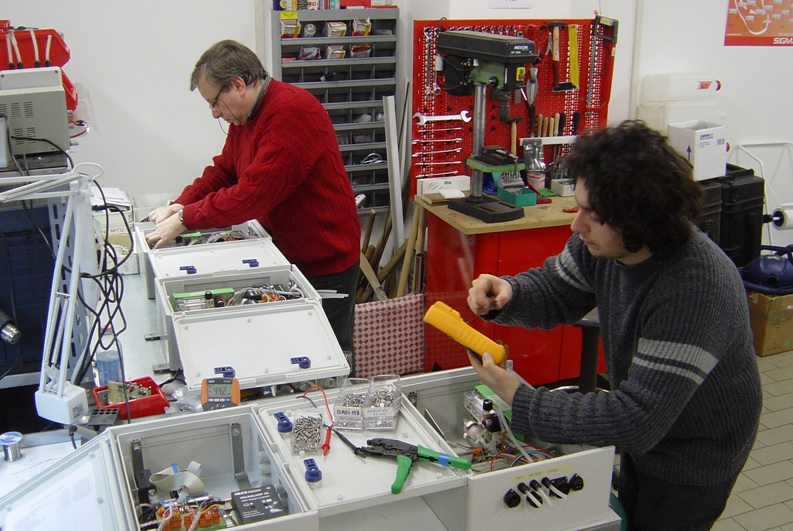
\includegraphics[scale=0.3]{Page1.png}}
		\end{center}
	\end{frame}
	
	\begin{frame}{\textbf{I valori della start-up}}
		\begin{itemize}
			\item Spesso questo genere di strumenti e di tecnologie sono state adottate da persone con competenze non tecniche per rispondere ad esigenze più artistiche che funzionali
			\item L'utilizzo degli stessi strumenti da parte di persone con esperienza nell'ambito tecnico permette una cosciente costruzione di pezzi di ricambio che non portano i difetti progettuali delle parti originali.
		\end{itemize}
		\begin{center}
			\zoombox{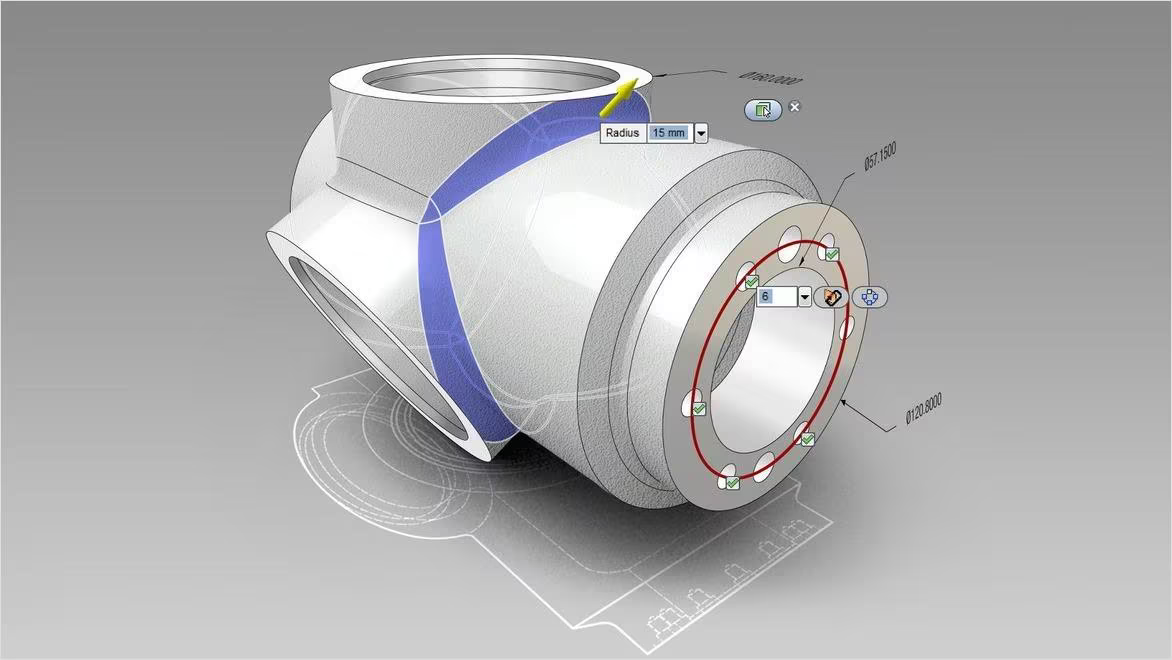
\includegraphics[scale=0.18]{Page2.png}}
		\end{center}
	\end{frame}
	
	\begin{frame}{\textbf{I valori della start-up}}
		\begin{itemize}
			\item Non c'è bisogno di seguire le logiche del consumismo, riparare gli oggetti non è solo una soluzione economica ma permette di ridurre la quantità di rifiuti. 
			\item Per essere ancora più ecosostenibili, dove possibile vengono usati materiali plastici biodegradabili come il PLA.
		\end{itemize} 
		\begin{tabularx}{\linewidth}{XX}
			{
				\begin{center}
					\zoombox{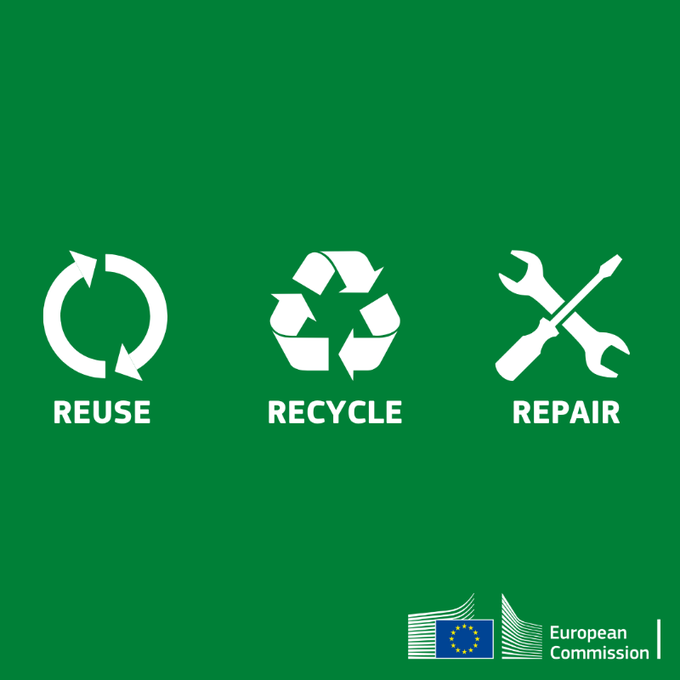
\includegraphics[scale=0.15]{Page31.png}}
				\end{center}	
			}&{
				\begin{center}
					\zoombox{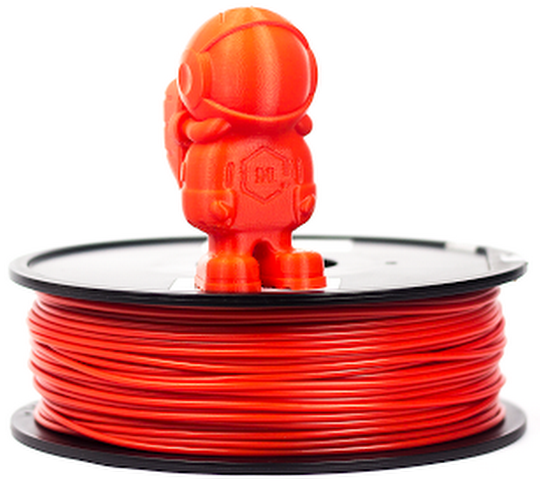
\includegraphics[scale=0.2]{Page32.png}}
				\end{center}
			}
		\end{tabularx}
	\end{frame}
	
	\begin{frame}{\textbf{I clienti di riferimento}}
		\begin{itemize}
			\item Le persone a cui è rivolto questo servizio sono i privati per piccole riparazioni o per la piccola produzione di gadget personalizzati ma sopratutto i centri di assistenza i quali potrebbero disporre di parti di ricambio per oggetti non più coperti dal produttore.
		\end{itemize}
		\begin{tabularx}{\linewidth}{XXX}
			{
				\begin{center}
					\zoombox{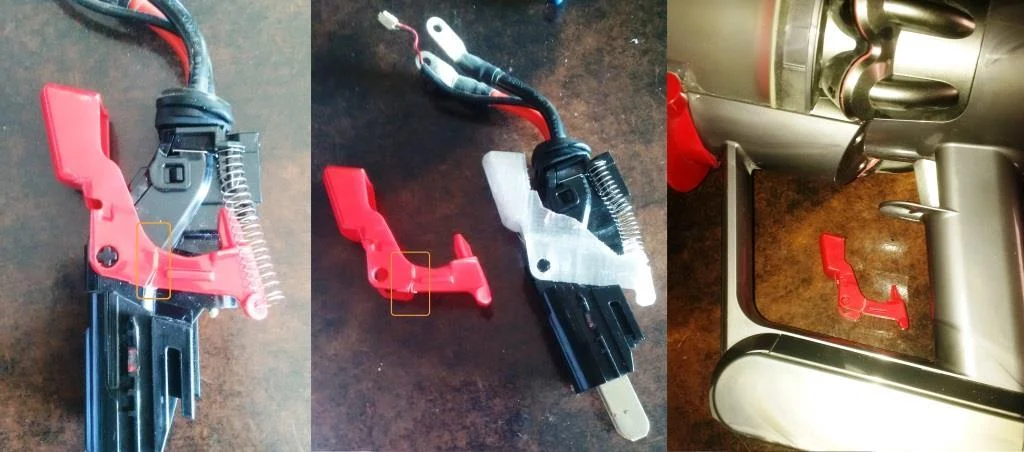
\includegraphics[scale=0.145]{Page41.png}}
				\end{center}
			}&{
				\begin{center}
					\hspace*{4mm}
					\zoombox{
\includegraphics[scale=0.15]{Page42.png}}
				\end{center}
			}&{
				\begin{center}
					\zoombox{\includegraphics[scale=0.07]{Page43.png}}
				\end{center}
			}
		\end{tabularx}
	\end{frame}

		\begin{frame}
			\maketitle
			\vspace*{-20mm}
			\begin{center}
				\vspace*{5mm}
				%\newline 
				\begin{tabularx}{\linewidth}{XX}
					{
						\hspace*{40mm}
						\zoombox{\includegraphics[scale=0.2]{logo_bianco.png}}
					}&{
						%\hspace*{10mm}
						\zoombox{
\includegraphics[scale=0.2]{logo-uniurb-2016.jpg}}
					}
				\end{tabularx}
			\end{center}
		\end{frame}
	
\end{document}